\section{Stima intervallare}\linkdest{interval}

\subsection{Credibility intervall (bayesiano) e Confidence interval (frequentista)}

\begin{frame}[fragile]{Bayesian credibility Interval}
\begin{block}{Credibility (della posterior)}
\begin{align*}
&\cred{(x)}=\int_{\mu\in\inf(x)}\Pi(\mu|x)\,d\mu=\int_{\mu\inf(x)}\frac{\prob{(x|\mu)}\prob{(\mu)}}{\int\,d\mu}\,d\mu>\cl{}\\
&
\end{align*}
\end{block}
\begin{block}{Ordinamento}
\begin{picture}(100,130)
\put(20,20){
\begin{tikzpicture}[scale=0.4]
\def\basefunc{exp(-(x-1)^2)}
        \begin{axis}[title={central},name=central,samples=50,ymin=0,xmin=-2,xmax=4,xlabel={$m$},ylabel={$\prob{(m|x_0)}$}]
        \addplot gnuplot [no marks,domain={-2:0}]{\basefunc} \closedcycle; 
        \addplot gnuplot [no marks,domain={2:4}]{\basefunc} \closedcycle; 
        \addplot gnuplot [black,thick,fill=grey,smooth,no marks,domain={0:2}]{\basefunc} \closedcycle;
        \node (unomenocl) at (axis cs:-1,0.3) {$1-\frac{\alpha}{2}$};
        \end{axis}
        \begin{axis}[title={upper limit}, at={($(central)+(4.5cm,-3cm)$)},name=upper,samples=50,ymin=0,xmin=-2,xmax=4,xlabel={$m$},ylabel={$\prob{(m|x_0)}$}]
        \addplot gnuplot [no marks,fill=grey,domain={-2:2}]{\basefunc} \closedcycle; 
        \addplot gnuplot [black,thick,smooth,no marks,domain={2:4}]{\basefunc};   
        \end{axis}
        \edef\oprob{0.47}
        \begin{axis}[at={($(upper)+(4.5cm,-3cm)$)}, title={probability order},name=central,samples=50,ymin=0,xmin=-2,xmax=4,xlabel={$m$},ylabel={$\prob{(m|x_0)}$}]
        \addplot[name path=prob] gnuplot[grey,thick,smooth,no marks]{\oprob};
        \addplot[name path=gauss] gnuplot[black,thick,smooth,no marks]{\basefunc};
        \path [name intersections={of=gauss and prob ,by={Pa,Pb}}];
        \node[above left] at (Pa) {$x_-$} node[above right] at (Pb) {$x_+$};
        \pgfkeys{/pgf/fpu=true}
        \pgfmathparse{1-sqrt(-ln(\oprob))}
        \def\xleft{\pgfmathresult}
        \pgfmathparse{1+sqrt(-ln(\oprob))}
        \def\xright{\pgfmathresult}
        \pgfmathparse{1+sqrt(-ln(\oprob))}
        \pgfkeys{/pgf/fpu=false}
        \addplot gnuplot [no marks,fill=grey,domain={0.13:1.87}]{\basefunc} \closedcycle; 
        \node (unomenocl) at (axis cs:0,0.7) {$CL$};
        \end{axis}
    \end{tikzpicture}}
\end{picture}
\end{block}
\end{frame}

\begin{frame}{Neyman construction. Frequentist confidence intervals}
%reminder: banda confidenza con pgfplot/gnuplot
\begin{columns}[T]
\begin{column}{0.4\textwidth}
\begin{figure}
    \centering
    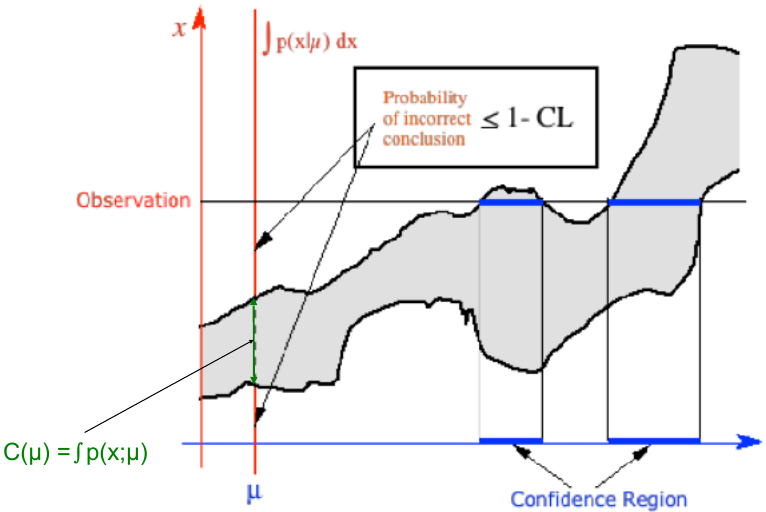
\includegraphics[width=0.9\textwidth,keepaspectratio]{clband}
    \label{fig:clband}
\end{figure}
\begin{figure}
    \centering
    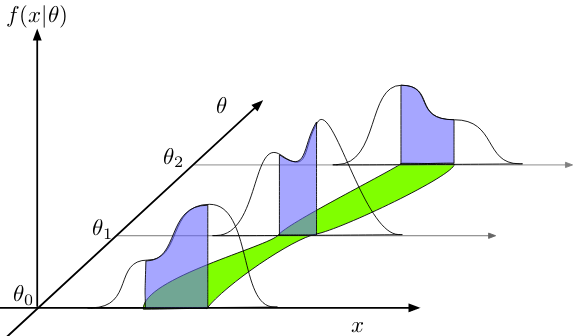
\includegraphics[width=0.9\textwidth,keepaspectratio]{neyman}
    \label{fig:neyman}
\end{figure}
\end{column}
\begin{column}{0.6\textwidth}
\begin{block}{Costruzione di Neyman}
Coverage: $\coverage{(\mu)}=\int_{x:\mu\in f(x)}\prob{(x:\mu)}\,dx$, $f(x)$ associa un intervallo nello spazio dei parametri a una misura; l'algoritmo ha livello di confidenza $\cl=\inf_{\mu\in A}C(\mu)$ cio\'e l'intervallo associato alla data misura ha probabilit\'a $\cl{}$ di contenere il parametro.
\end{block}
\begin{block}{Ordering}
''The way I integrate over the data''
\end{block}
\end{column}
\end{columns}
\end{frame}

\begin{frame}{Feldman-Cousins unified approach.}
\begin{columns}[T]
\begin{column}{0.5\textwidth}
insactisfaction with Neyman construction for upper limit in case of empty/unphysical interval (flip-flop problem depending on data)
\end{column}
\begin{column}{0.5\textwidth}
LR-ordering $R=\frac{\prob{(x;\mu)}}{\prob{(x;\mu_{best})}}$: values of x/n are added to acceptance region as decreasing function of R.
\end{column}
\end{columns}
\end{frame}

\begin{wordonframe}{Intervalli di confidenza per $U([0,m])$}
Una misura:
\begin{columns}[T]
	\begin{column}{0.5\textwidth}
\def\myscale{0.4}
\begin{tikzpicture}[myscalar]
\begin{axis}[title={Banda di credenza per $U([0,m])$},name=uniformcredence,ymin=0,xmin=0,xmax=6,xlabel={$m$},ylabel={$x$},y label style={rotate=-90, at={(-0.1,1.)}},extra x tick style={% changes for extra x ticks
	tick label style={yshift=-4mm}},
extra x tick labels={$x\exp{1-\alpha}$},extra y ticks={0.5},extra y tick labels={measure $x_0$}]
\addplot[name path global=om, no marks] gnuplot[id=upperbound,domain=0:6] {x};
\addplot[name path global=op, no marks] gnuplot[id=lowerbound,domain=0:6] {x*exp(-1+0.05)};
\addplot[name path global=meas,dash pattern=on 4pt off 3pt,no marks,samples=10,black,thin] gnuplot[domain=0:6] {0.5};
\end{axis}
\end{tikzpicture}

\def\myscale{0.4}
\begin{tikzpicture}[myscalar]
\begin{axis}[title={Banda confidenza $U([0,m])$},name=uniformconfidence,ymin=0,xmin=0,xmax=8,xlabel={$m$},ylabel={$x$},y label style={rotate=-90, at={(-0.1,1.)}},extra x tick style={% changes for extra x ticks
	tick label style={yshift=0mm}},extra y ticks={0.3},extra y tick labels={measure $x_0$}]
\addplot[name path global=bp, no marks] gnuplot[id=upperbound,domain=0:8] {x*(1-0.9)};
\addplot[name path global=bm, no marks] gnuplot[id=lowerbound,domain=0:8] {(x)};
\addplot[name path global=meas,dash pattern=on 4pt off 3pt,no marks,samples=10,black,thin] plot[domain=0:8] {0.3};
\path[name intersections={of={bp and meas},name=i},name intersections={of={bm and meas},name=j}] (i-1) (j-1);
\pgfplotsextra{\path (i-1)  \pgfextra{\markxof{i-1}\xdef\myfirsttick{\pgfmathresult}}(j-1) \pgfextra{\markxof{j-1}\xdef\mysecondtick{\pgfmathresult}};
}
\end{axis}
\draw[ultra thin, draw=gray] (i-1 |- {rel axis cs:0,0}) node[fill=yellow,yshift=0ex]{\pgfmathprintnumber[fixed,precision=5]\myfirsttick} -- (i-1);
\draw[ultra thin, draw=gray] (j-1 |- {rel axis cs:0,0}) node[fill=red]{\pgfmathprintnumber[fixed,precision=5]\mysecondtick} -- (j-1);
\end{tikzpicture}
\end{column}
\begin{column}{0.5\textwidth}
La banda di confidenza si costruisce integrando sulla distribuzione dell'osservabile su una regione tale che l'integrle sia il livello di confidenza $\cl=1-\alpha$.

L'intervallo di credibilit\'a \'e definito dalla banda per cui 

\end{column}
\end{columns}
\end{wordonframe}

\subsection{Pivotal quantities}

\begin{frame}{Pivot}
Pivot: RV $U(T,\theta)$ funzione dib statistica sufficiente e parametro ma la distribuzione di U non dipende dal parametro $\forall \theta\in\Theta$ (asymptotic if true for $n\to\infty$).
\begin{align*}
&p(x;\mu)=\frac{1}{\sqrt{2\pi}\sigma}\exp{-\frac{(x-\mu)^2}{2\sigma^2}}\\
&(s=\frac{x-\mu}{\sigma}:\ p(s;\mu)=N(0,1)\\
&\int_{s>c}p(s)\,DS=\cl{}
\end{align*}
\mykeyword{Pivot. 2-sided CI for exponential}:
\begin{align*}
&f(x;\theta)=\invers{\theta}\exp{-\frac{x}{\theta}}I(x>0)\ \to\ g(u)=\exp{-u}I(u>0)\\
&\prob{(a<u<b)}=1-\alpha\Rightarrow\prob{(\theta\in(\invers{b}x,\invers{a}x))}=1-\alpha\ (\alpha\leftrightarrow1-\alpha)\\
&
\end{align*}
\end{frame}

\begin{frame}{Teorema di Wilks}
$p(x;\mu)$ due volte differenziabile con dominio indipendente da parametro $\Omega(x;\mu)=\Omega(x)$: \[\lambda(x;\mu)=2\log{[\frac{\sup_{\mu}{p(x;\mu)}}{p(x;\mu)}]}\] (log-likelihood ratio statistics) ha asintoticamente pdf universale e indipendente da $\mu$: distribuzione di $\chi^2$ con dof pari a dimensione di $\vec{\mu}$.
\begin{align*}
&\ln{L(\theta)}-\ln{L(\hat{\theta})}=-\frac{1}{2}\invers{F}_{\chi_n^2}(1-\alpha)
\end{align*}
\end{frame}

\begin{wordonframe}{Esempi intervalli di confidenza e credibilit\'a}
\begin{block}{Limite superiore Poisson con $k=0$}
$\prob{(k|\mu)}=\frac{\mu^k\exp{-\mu}}{k!}$: registro $k=0$ conteggi, ricavo limite superiore frequentista e bayesiano per $\mu$
\end{block}

\mykeyword{Ex: limite superiore bayesiano per Poisson} - La posterior $\prob{(\mu|0)}=\exp{-\mu}$ per $\cl{}=\alpha\%$ si ha $\int_0^{\mu_u}\exp{-\mu}\,d\mu=\alpha$, per $\cl{}=90\%$ si ha $\mu<2.3@90\%\cl{}$.
\begin{columns}[T]
\begin{column}{0.5\textwidth}
\mykeyword{Ex: limite superiore frequentista per Poisson} - Upper limit: $\sum_{k_{min}}^{\infty}\prob{(k|\mu)}=\alpha$; $\prob{(0|\mu)}=0.1 (=1-\alpha)$ per $\mu_0=\ln{10}$, $\prob{(0|\mu_1)}+\prob{(1|\mu_1)}=0.1$ per $\mu_1=3.89$, $\prob{(0|\mu_1)}+\prob{(1|\mu_1)}+\prob{(2|\mu_1)}=0.1$ per $\mu_2=5.32$
\end{column}
\begin{column}{0.5\textwidth}
\begin{picture}(100,130)
\put(20,20){
	\begin{tikzpicture}[scale=0.4]
	\begin{axis}[title={Coverage},name=central,samples=50,ymin=0,xmin=0,xmax=6,xlabel={$\mu$},ylabel={$k$},y label style={rotate=-90, at={(-0.1,1.)}},extra x ticks={2.3,3.89,5.32},extra x tick style={% changes for extra x ticks
		tick label style={yshift=-4mm}},
	extra x tick labels={$\mu_0$, $\mu_1$, $\mu_2$},extra y ticks={0},extra y tick labels={measure $k=0$}]
	\addplot+[name path=dwcover,const plot, no marks, thick] coordinates {(0,0) (2.3,1) (3.89,2) (5.32,3)};
	\addplot[quiver={u=0,v=x>2.3 ? (x>3.9 ? -1 : -2):-3},-stealth, samples=15] {3}; 
	\end{axis}
	\end{tikzpicture}}
\end{picture}	
\end{column}
\end{columns}

\mykeyword{Ex: Poisson con $k=0,1,2$ conteggi e ordinamento LR, Up, Down, Central} -

\mykeyword{Ex: Limiti bayesiani e frequentisti sul numero di facce dadi D\&D estrazioni 1,1} - $S=\{4,6,8,10,12,20\}$:
\begin{columns}[T]
\begin{column}{0.5\textwidth}
 \mykeyword{T bayes (lancio 6 dadi)} $\pgfkeys{/pgf/fpu=true}\prob{(1)}=\sum_i\prob{(D_i)}\prob{(1|D_i)}=\xdef\Sum{0}
\foreach \i in {4,6,8,10,12,20} {\xdef\Sum{\Sum+1/(6*\i)}}\pgfmathparse{\Sum}\pgfmathprintnumber{\pgfmathresult}\pgfkeys{/pgf/fpu=false}$
Limite superiore al numero di facce: $\sum_{\mu}\prob{(x_0;\mu)}\geq1-\alpha$, $n_f\leq12$ at $\cl>90\%$
\end{column}
\begin{column}{0.5\textwidth}
\pgfkeys{/pgf/fpu=true}
\pgfmathparse{(1/4)*(1/6)*(1/0.1292)}\pgfmathsetmacro{\postfour}{\pgfmathresult}
\pgfmathparse{(1/6)*(1/6)*(1/0.1292)}\pgfmathsetmacro{\postsix}{\pgfmathresult}
\pgfmathparse{(1/8)*(1/6)*(1/0.1292)}\pgfmathsetmacro{\posteight}{\pgfmathresult}
\pgfmathparse{(1/10)*(1/6)*(1/0.1292)}\pgfmathsetmacro{\postten}{\pgfmathresult}
\pgfmathparse{(1/12)*(1/6)*(1/0.1292)}\pgfmathsetmacro{\posttwelve}{\pgfmathresult}
\pgfmathparse{(1/20)*(1/6)*(1/0.1292)}\pgfmathsetmacro{\posttwenty}{\pgfmathresult}
\pgfkeys{/pgf/fpu=false}
\begin{tikzpicture}[scale=0.5]
\begin{axis}[
ybar stacked,
bar width=15pt,
nodes near coords% = {%
%\pgfmathprintnumberto[fixed,assume math mode=true]{\pgfplotspointmeta}{\myval}%
%\pgfmathparse{\myval<0.05?:\myval}\pgfmathresult%}
,
enlargelimits=0.2,
ylabel={$\prob{(D_i|1)}$},
symbolic x coords={d4, d6, d8, d10, d12, d20},
xtick=data,
x tick label style={anchor=north},
xticklabels={$D_4$, $D_6$, $D_8$, $D_{10}$, $D_{12}$, $D_{20}$},cycle list name = ColorListBar
]
\addplot+[ybar] plot coordinates {(d4,\postfour) (d6,\postsix) (d8,\posteight) (d10,\postten) (d12,\posttwelve) (d20,\posttwenty)};
\end{axis}
\end{tikzpicture}
Probability ordering (Cosa vuol dire ordinamento?)
\end{column}
\end{columns}
\begin{columns}[T]
	\begin{column}{0.3\textwidth}
\begin{tikzpicture}[scale=0.3]
\begin{axis}[
ybar stacked,
bar width=15pt,
nodes near coords% = {%
%\pgfmathprintnumberto[fixed,assume math mode=true]{\pgfplotspointmeta}{\myval}%
%\pgfmathparse{\myval<0.05?:\myval}\pgfmathresult%}
,
enlargelimits=0.2,
ylabel={$\prob{(D_i)}$},
symbolic x coords={d4, d6, d8, d10, d12, d20},
point meta=explicit symbolic,
xtick=data,
ytick={4,6,8,10,12,20},
x tick label style={anchor=north},
xticklabels={$D_4$, $D_6$, $D_8$, $D_{10}$, $D_{12}$, $D_{20}$},cycle list name = ColorListBar,every node near coord/.append style={font=\tiny}
]

\addplot+[ybar] plot coordinates {(d4,4)[$1/4$] (d6,4) [$4/6$]
	(d8,4)[$4/8$] (d10,4)[$4/10$] (d12,4)[$4/12$] (d20,4)[$4/20$]};
\addplot+[ybar] plot coordinates {(d4,16)[$0$] (d6,2) [$1$]
	(d8,2)[$6/8$] (d10,2)[$6/10$] (d12,2)[$6/12$] (d20,2)[$6/20$]};
\addplot+[ybar] plot coordinates {(d4,0)[$0$] (d6,14) [$0$]
	(d8,2)[$1$] (d10,2)[$8/10$] (d12,2)[$8/12$] (d20,2)[$8/20$]};
\addplot+[ybar] plot coordinates {(d4,0)[$0$] (d6,0) [$0$]
	(d8,12)[$0$] (d10,2)[$1$] (d12,2)[$12/10$] (d20,2)[$20/10$]};
\addplot+[ybar] plot coordinates {(d4,0)[$0$] (d6,0) [$0$]
	(d8,0)[$0$] (d10,10)[$0$] (d12,2)[$1$] (d20,2)[$20/12$]};
\addplot+[ybar] plot coordinates {(d4,0)[$0$] (d6,0) [$0$]
	(d8,0)[$0$] (d10,0)[$0$] (d12,8)[$0$] (d20,8)[$1$]};
\end{axis}
\end{tikzpicture}
\end{column}
	\begin{column}{0.7\textwidth}
limiti di confidenza frequentisti: costruzione banda di confidenza prendendo ordinamento sulla pdf di X a parametro dato. Limite superiore ordinando da 20 per estrazione 1 si ha $n_f\leq8$ con $\cl{}\geq90\%$
\end{column}
\end{columns}
\mykeyword{Ex: Dadi D\&D CI frequentista con LR ordering}
\end{wordonframe}

\section{Test di ipotesi}\linkdest{test}

\begin{frame}{Testing simple hypothesis}

\begin{block}{Test: funzione dallo spazio delle osservabili in H.}
Un'ipotesi \'e un'affermazione sui parametri che caratterizzano lo stato della natura; se l'ipotesi non \'e sufficienta a determinare distribuzione di probabilit\'a della nostra osservabile l'ipotesi \'e composta: se ipotesi da falsificare \'e non esistenza higgs ($m=0$) semplice, ma alternativa \'e composta da $m>0$
\end{block}

\begin{block}{Regione critica(C)/di accettazione($\overline{C}$) nello spazio delle X}
Due sottoinsiemi di X individuano la regione critica e regione di accettazione (conferma $H_0$).
\end{block}

\end{frame}

\begin{frame}{Propriet\'a dei test. MP test.}
\begin{block}{errore tipo I/II}
	\begin{itemize}
		\item Errore di tipo I (falso positivo), scarto $H_0$ quando \'e vera (loss,size,taglia,livello di significativit\'a $1-\alpha$: $\alpha=\prob{(x\in C|H_0)}=\prob_0{(x\in C)}$.
		\item Errore tipo II (falso negativo, contaminazione): probabilit\'a di accettare erroneamente $H_0$, $\prob{(x\in\overline{C}|\not{H_0})}=\beta$. Potenza del test $1-\beta$ \'e la capacit\'a di distinguere ipotesi diverse da $H_0$ 
	\end{itemize}
\end{block}

\begin{block}{Propriet\'a dei test}
	\begin{itemize}
		\item Consistenza: ($\lim_{n\to\infty}{(\pow{(i)})}=1$ per ogni $i\neq0$: se prendo infiniti dati distinguo $H_1$ da $H_0$, non \'e detto che sia uniforme.
		\item unbiasedness $\pow{}\geq\alpha, \forall i$, T consistente \'e asintoticamente unbiased
	\end{itemize}
\end{block}
 \begin{block}{Ottimizzazione: power maggiore possibile.}
UMP test: power maggiore uguale a qualunque test per tutte le ipotesi: esiste?
\end{block}
\end{frame}

\begin{frame}{Lemma di Neyman-Pearson}
\begin{block}{Statistica di un test}
Posso esprimere un test in funzione di una statistica: $T(\vec{x})=T(t(\vec{x}))$ (nel caso del lemma NP la statistica \'e il LR). 
\end{block}
Fisso ipotesi singola $i_0$ l'MP test \'e quello che mi da come regione critica gli x tali che $\frac{\prob_0{(x)}}{\prob_1{(x)}}<q(\alpha)$, $q$ \'e determinato da condizione $\prob{(C|H_0)}\leq\alpha$ (LR), questo \'e il test di massimo power.

\end{frame}

\begin{wordonframe}{Dimostrazione lemma Neyman-Pearson}
Per ogni test alternativo $T'$ prendo $\alpha'\leq\alpha_{NP}$ allora $\beta'\geq\beta_{NP}$ ($\pow'\leq\pow_{NP}$, probabilit\'a errore tipo II \'e maggiore), dimostro $\beta'-\beta\geq0$ cio\'e $\prob{(\overline{C}'|H_1)}-\prob{(\overline{C}|H_1)}$:
\begin{align*}
&\prob{(C|H_1)}-\prob{(C'|H_1)}=\prob{(C\cap|H_1)}+\prob{(C\cap\overline{C}'|H_1)}-\prob{(C\cap C'|H_1)}-\prob{(C'\cap\overline{C}|H_1)}=\prob{(C\cap\overline{C}'|H_1)}-\prob{(C'\cap\overline{C}|H_1)}\\
&\prob{(C\cap C'|H_1)}=\int_{C\cap C'}\prob_1{(x)}\,dx\geq\int_{C\cap \overline{C}'}\frac{\prob_0{(x)}}{q}\,dx=\frac{1}{q}\prob{(C\cap\overline{C}'|H_0)}
\end{align*}
\end{wordonframe}

\begin{frame}{Test UMP unilaterale per famiglia esponenziale: Karlin-Rubin theorem.}
	Esiste UMP test per distinguere $H_0: \mu\leq\mu_0$, $H_{\mu}: \mu>\mu_0$ - se il likelihood ratio \'e funzione monotona di una statistica $T(\vec{X})$ e scelgo $\alpha$ e $k_{\alpha}$ tali che $\prob{(T(x)\geq k_{\alpha})}=\alpha$  allora la regione critica per un test UMP unilaterale $H_0$ vs $H_1$ \'e $C=\{x:T(x)\geq q_{\alpha}\}$; per pdf della froma $\prob{(x,\mu)}=F(x)G(\mu)\Exp{[A(x)B(\mu)]}$ e $B(\mu)$ crescente il rapporto di likelihood \'e monotono e la statistica del test \'e $\sum_iA(x_i)$
\[\frac{F(x)G^N(\overline{\mu})}{F(x)G^N(\overline{\mu}_0)}\Exp{[\sum_iA(x_i)](B(\overline{\mu})-B(\overline{\mu}_0))}\]
$F,G>0$.
\cite[5]{lrtmptumpt}; \cite[445]{inferencemukhopadhyay2000}
\end{frame}

\begin{wordonframe}{Test examples}
	\begin{block}{Power}
plot power(i) parte da $\alpha$ e va a 1 al crescere di i (separazione ipotesi) e pi\'u rapidamente al crescer di N.
	il grafico del power ($\prob{(\text{reject} H_0)| H_i}$) in funzione dell'indice i che identifica le ipotesi (per $H_0$ fa $\beta=1-\alpha$ quindi il power \'e $\alpha$) allontanandosi da $H_0$ deve essere il pi\'u grande possibile. 
\end{block}
\begin{block}{grafico $\prob_0{(X)}$ vs $\prob_1{(X)}$ con definizione di regione critica}
\begin{picture}(100,130)
\put(20,20){
	\begin{tikzpicture}[scale=0.3]
	\begin{axis}[title={Regione critica/accettanza per $H_0$},name=testh0,samples=100,ymin=0,xmin=0,xmax=10,xlabel={$x$},ylabel={$\prob{(x)}$},extra x ticks={1.3},extra x tick style={% changes for extra x ticks
		tick label style={yshift=-4mm}},
	]
	\addplot[id=aa] gnuplot {(sqrt(2*pi))^(-1)*exp(-(x-2)^2/(2))};
	\addplot[id=bb,domain=0:10] gnuplot {(2*sqrt(2*pi))^(-1)*exp(-(x-6)^2/(2*4))}; 
	\end{axis}
	\end{tikzpicture}
}
\end{picture}
\end{block}
\end{wordonframe}

\begin{wordonframe}{LMP tests. LRT.}
(LMP) Se ho bisogno di massima sensibilit\'a vicino alla soglia: $1-\beta$ grande nelle vicinanze di 0, $L(\mu)\approx L(0)+\PDy{\mu}{L}|_0\mu+\ldots$ $\log{L(\mu)}\approx \log{L}(0)+\PDy{\log{\mu}}{L}|_0\mu+\ldots$: $L(\mu)=L(0)\Exp{[\PDy{\mu}{\log{L}}\mu]}$ $(A(x)B(\mu))$: $t(x)=\PDy{\mu}{\log{L}}|_{\mu=0}=S(x)$ (lo score \'e asintoticamente normale Test a $n\sigma$ $q_{\alpha}=n\sqrt{I_{tot}}$).
\end{wordonframe}

\begin{wordonframe}{Max power test in intervallo}
\begin{itemize}
\item \'E possible espansione L in intervallo?
\item Metodo empirico del LR. Uso stimatore ML $\hat{\mu}$: $t_{NP}=\frac{L(H_0)}{L(H_{\mu})}$. Introduco $\lambda=2\log{\frac{\sup_{\mu}}{L(\mu_0)}}$; Ipotesi complesse: $H_0: p(x;\mu_0,\nu)$ $H_{\mu}: p(x;\mu,\nu)$, $\prob{(\lambda)}\to \chi^2_{\dim{\mu-\nu}}$
\end{itemize}
\end{wordonframe}

\begin{frame}{Propriet\'a $\chi^2$}
La distribuzione di chi-squared con $\nu$ gradi di libert\'a $\prob{(\chi_{\nu}^2)}$ \'e la distribuzione di probabilit\'a di $\sum_1^{\nu}x_i^2$ con $x_i\to N(0,1)$, $\chi^2$ non centrale $x_i\to N(\mu_i,1)$, parametro non centralit\'a $\lambda=\sum\mu_i^2$.
\begin{columns}[T]
\begin{column}{0.7\textwidth}
Momenti:
\begin{align*}
&\phi_1(t)=\E_{\chi^2_1}{(\exp{it\chi^2})}\\
&=\E_x{\exp{itx^2}}=2\frac{p(x)}{|\TDy{x}{y}|}=\intsinf{}\frac{\exp{itx-x^2/2}}{\sqrt{2\pi}}\,dx\\
&=\frac{1}{\sqrt{1-2it}},\ \phi_{\chi^2_{\nu}}(t)=(1-2it)\expy{-\frac{\nu}{2}}\\
&
\end{align*}
\end{column}
\begin{column}{0.3\textwidth}
\begin{align*}
&\E{(\chi^2_{\nu})}=\nu\\
&\var{[\chi_{\nu}^2]}=2\nu\\
&\E{(\chi^{2,NC}_{\nu})}=\nu+\lambda
\end{align*}
\end{column}
\end{columns}
\begin{align*}
&\prob{(x=\chi^2_{\nu})}=\frac{1}{2\expy{\nu/2}\Gamma(\frac{\nu}{2})}x\expy{\frac{\nu}{2}-1}\exp{-\frac{x^2}{2}}\\
&\lim_{\nu\to\infty}N(\nu,2\nu)
\end{align*}
Approssimazione di Fisher: $\prob{(\sqrt{2\chi^2})}\approx N(\sqrt{2\nu-1},1)$
\end{frame}
